\section{Higgs zero mode II: reduced model, resonance and width}\label{rep:h-reduced}

We solve the zero-mode problem of Sec.~\ref{rep:h-matching} in a model with two coordinates, the Higgs radius $r$ and the modulus $s=|\bm w|$ of the hypercharge zero mode, with the SU(2) zero modes in a conditional Gaussian.
We show that the Gaussian factorizes exactly, that the hypercharge zero mode is not fast where the Higgs zero mode sits and must be treated jointly with $r$, and that the resulting two-dimensional model reproduces the full sixteen-dimensional ground state at $\lambda=0$ to $0.003/L$. %
For $\lambda<0$ the electroweak state is a finite-volume resonance with complex energy $E=\varepsilon-i\Gamma/2$; we compute $\Gamma$ as a multichannel Siegert state and confirm it with absorbing potentials and real-wall stabilization.
Full-dimensional diffusion Monte Carlo (DMC) with a gauge-invariant wall confirms the resonance energy to $0.005/L$, and four independent estimates give the same width to within $8\%$.
Together they would raise the critical top mass by $+0.005\GeV$ at $\Pone=0.9$ and $+0.008\GeV$ at $\Pone=1/2$ (Sec.~\ref{rep:v-fulldim}); the central values do not include this shift, which lies inside the one-sided full-dimensional item of the error budget. %
Finally we explain the size of the threshold: near threshold $\ln\Gamma=a-b|\lambda|^{-1/2}$, and the closed form $|\lamc|^{1/2}\simeq b_{\rm eff}/\ln(A_{\rm eff}\eta_\infty/\ln2)$, with the effective slope $\sigma_{\rm eff}=0.44$ and the prefactor $A_{\rm eff}\simeq310$ fixed by the computed threshold, shows that the confinement slope sets the size of $\lamc$ and that the duration of the turn enters only logarithmically. %
Under assumption (A5) of Sec.~\ref{rep:setup} the zero-mode dynamics is that of this model, with the residual errors collected in Sec.~\ref{rep:h-budget}.

\subsection{Conditional Gaussian of the gauge zero modes and its exact factorization}
\label{sec:rb-gauss}

At fixed $r$ we take the state of the gauge zero modes from the most general central Gaussian that is invariant under spatial rotations and residual U(1)$_{\rm em}$.
Different spatial directions are uncorrelated, because a two-point function of spatial vectors can only be proportional to $\delta_{ij}$.
In each direction the precision matrix on $y_i=(x_i^1,x_i^2,x_i^3,w_i)$ is ${\rm diag}(a,a,K_2)$, where U(1)$_{\rm em}$ invariance forces the two charged components $x^{1,2}$ to share one parameter $a$ and decouple, and
\begin{equation}
K_2=\begin{pmatrix}k&c\\ c&e\end{pmatrix},\qquad D=ke-c^2 .
\label{eq:rb-K2}
\end{equation}
(The parameter $c$ of $K_2$ is a Gaussian parameter, not the holonomy of Sec.~\ref{sec:rb-r2c2}.)
Completing the square in the neutral block,
\begin{equation}
k\,(x^3)^2+2c\,x^3w+e\,w^2=k\,(x^3+\beta w)^2+\tilde e\,w^2,\qquad \beta=\frac ck,\qquad \tilde e=e-\frac{c^2}{k},
\label{eq:rb-square}
\end{equation}
so the Gaussian factorizes exactly into a conditional state of the SU(2) modes and a marginal state of the hypercharge mode,
\begin{align}
\Psi&=\varphi(\bm x|\bm w)\,\chi(\bm w),\qquad \chi\propto e^{-\tilde e\,|\bm w|^2/2},\nonumber\\
\varphi&\propto \prod_i \exp\Bigl\{-\tfrac12\Bigl[a\bigl((x_i^1)^2+(x_i^2)^2\bigr)+k\bigl(x_i^3+\beta w_i\bigr)^2\Bigr]\Bigr\}.
\label{eq:rb-condGauss}
\end{align}
For $\psi\propto\exp(-\frac12y^{\mathsf T}Ky)$ one has $\langle p_ip_j\rangle=K_{ij}/2$ and $\langle y_iy_j\rangle=(K^{-1})_{ij}/2$, and all moments of Eq.~(\ref{eq:rb-H0}) are elementary~\cite{Luscher:1982ma,vanBaal:2000zc}:
\begin{align}
\bigl\langle\tfrac12p^2\bigr\rangle&=\tfrac34(2a+k+e),\nonumber\\
\bigl\langle\tfrac12y^{\mathsf T}\mathcal My\bigr\rangle&=\frac{3r^2}{16}\Bigl[\frac{2g_2^2}{a}+\frac{g_2^2e-2g_2g_Yc+g_Y^2k}{D}\Bigr],\nonumber\\
\Bigl\langle\frac{g_2^2}{4}\sum_{ij}|\bm x_i\times\bm x_j|^2\Bigr\rangle&=\frac{3g_2^2}{4a^2}+\frac{3g_2^2e}{2aD},\nonumber\\
\frac{2}{r^2}\bigl\langle(L^1)^2+(L^2)^2\bigr\rangle&=\frac{3}{ar^2}\,\frac{e(k-a)^2-2c^2(k-a)+kc^2}{D},
\label{eq:rb-moments}
\end{align}
where $\mathcal M$ is the mass matrix of Eq.~(\ref{eq:rb-massmatrix}) and the last line follows from $L^1\chi=i\,x^2[(k-a)x^3+cw]\chi$, the action of an SU(2) rotation about the 1-axis on the Gaussian.
In terms of $\beta$ and $\tilde e$ the sum of the four moments takes the form
\begin{align}
E_{\rm tot}&=C_0+\frac34\Bigl(\tilde e+\frac{\Omega^2}{\tilde e}\Bigr),\nonumber\\
\Omega^2&=\frac{r^2}{4}(g_Y-g_2\beta)^2+\frac{2g_2^2\beta^2}{a}+\frac{4a\beta^2}{r^2},
\label{eq:rb-Etot}
\end{align}
with
\begin{equation}
C_0=\tfrac34(2a+k)+\tfrac34k\beta^2+\frac{3r^2}{16}\Bigl(\frac{2g_2^2}{a}+\frac{g_2^2}{k}\Bigr)+\frac{3g_2^2}{4a^2}+\frac{3g_2^2}{2ak}+\frac{3(k-a)^2}{akr^2}.
\label{eq:rb-C0}
\end{equation}
The three terms of $\Omega^2$ come from the Higgs mass term, in which $x^3=-\beta w+\delta x^3$ leaves $(g_Y-g_2\beta)w$ in the massive combination, from the magnetic quartic, and from the angular term of Eq.~(\ref{eq:rb-bodyframe}).
The hypercharge mode is a harmonic oscillator of frequency $\Omega$, so the minimization over $\tilde e$ gives $\tilde e=\Omega$ and $E_{\rm tot}=C_0+\frac32\Omega$.
We minimize over the remaining parameters $(a,k,\beta)$ globally from many starting points and by Newton continuation in $r$; at six radii the global minima agree with the continuation to $4\times10^{-15}$. %

\paragraph{Born--Huang term.}
When the gauge state follows $r$ adiabatically, the radial motion acquires the Born--Huang term $B_r=\frac12\langle\partial_r\Psi|\partial_r\Psi\rangle=\frac{3}{16}{\rm tr}[(K^{-1}K')^2]$, with $K'$ obtained by implicit differentiation of the stationarity conditions rather than by differences.
It splits exactly into
\begin{align}
B_x&=\frac{3}{16}\Bigl[2\Bigl(\frac{a'}{a}\Bigr)^2+\Bigl(\frac{k'}{k}\Bigr)^2\Bigr],\qquad
B_w=\frac{3}{16}\Bigl(\frac{\tilde e'}{\tilde e}\Bigr)^2,\nonumber\\
B_\beta&=\frac{3k\beta'^2}{8\tilde e}=\Bigl\langle\frac k4\beta'^2|\bm w|^2\Bigr\rangle_\chi .
\label{eq:rb-BH}
\end{align}
At small $r$ the mass term dominates $\Omega$, $\tilde e=\Omega\simeq g_Yr/2$, and therefore
\begin{equation}
B_w=\frac{3}{16}\Bigl(\frac{\Omega'}{\Omega}\Bigr)^2\xrightarrow{\;r\to0\;}\frac{3}{16r^2};
\label{eq:rb-Bw}
\end{equation}
numerically $r^2B_w=0.1875000$ at $r=0.004$. %
The moments, the factorization, and Eqs.~(\ref{eq:rb-C0})--(\ref{eq:rb-BH}) were rederived symbolically with Gaussian expectation values in Wolfram Language; the six identities vanish identically and hold numerically to $10^{-14}$ at all $r$. %

\paragraph{The hypercharge zero mode is not fast.}
A term $3/(16r^2)$ is as singular as the centrifugal term $3/(8r^2)$ and would raise the Frobenius exponent of the radial function from $3/2$ to $1.6726$ [from $s_0(s_0-1)/2=\frac38+\frac3{16}$]. %
Its origin is unphysical: the hypercharge oscillator has frequency $\Omega\propto r$, so it is soft exactly where the Higgs zero mode sits, and the adiabatic assumption fails there.
Table~\ref{tab:rb-BH} shows the consequences in the $\lambda=0$ ground state of the two-dimensional model below.
$B_w$ is $0.44$ at $r=0.65$ and $0.18$ at $r=1$; the exact conditional width $\langle s^2\rangle$ saturates near $5$, whereas the adiabatic value $3/(2\Omega)$ grows to $11$--$17$ at $r=0.4$--$0.6$, which softens the inner wall. %
In the barrier region, $r\approx3$--$5.5$, $B_w<0.006$ is smaller than $B_x$ and $B_\beta$, and $\bm w$ follows its local ground channel. %
Beyond $r\approx2$ the soft direction turns from $\bm w$ into the photon combination: $\beta$ grows from $0.1$ to $0.76$. %
A one-dimensional Born--Oppenheimer reduction in $r$ is therefore unreliable in the well and adequate under the barrier.

\begin{table}[t]
\centering
\caption{Born--Huang terms and conditional width of the hypercharge mode in the $\lambda=0$ ground state of the two-dimensional model, compared with the Born--Oppenheimer width $3/(2\Omega)$; the last column is the radial probability density.} %
\label{tab:rb-BH}
\begin{tabular}{ccccccc}
\toprule
$r$ & $\Omega$ & $B_x$ & $B_w$ & $\langle s^2\rangle$ & $3/(2\Omega)$ & $\rho(r)$ \\
\midrule
$1.0$ & $0.219$ & $0.0024$ & $0.176$ & $4.90$ & $6.79$ & $0.51$ \\ %
$1.5$ & $0.320$ & $0.0048$ & $0.066$ & $4.55$ & $4.65$ & $0.68$ \\ %
$2.0$ & $0.407$ & $0.0075$ & $0.028$ & $4.15$ & $3.60$ & $0.46$ \\ %
$3.0$ & $0.530$ & $0.0115$ & $0.0053$ & $3.49$ & $2.79$ & $0.05$ \\ %
\bottomrule
\end{tabular}
\end{table}

\subsection{The two-dimensional Hamiltonian}
\label{sec:rb-2d}

We keep $\varphi(\bm x|\bm w)$ at the pointwise optimal parameters and replace $\chi(\bm w)$ by a function $\chi(r,\bm w)$ that we solve for.
Because $\varphi$ is real and normalized, $\langle\varphi|\partial\varphi\rangle=0$, the cross terms of the kinetic energy vanish, and the projection onto the trial family $\chi(r,\bm w)\varphi(\bm x|r,\bm w)$ is exact: $\frac12\langle|\partial_{\bm w}\varphi|^2\rangle=\frac34k\beta^2$ is part of $C_0$, and $\frac12\langle|\partial_r\varphi|^2\rangle=B_x+\frac k4\beta'^2|\bm w|^2$ adds to the stiffness of $\bm w$.
Acting on $u=r^{3/2}f$, the model Hamiltonian is
\begin{align}
H_{\rm 2D}={}&-\tfrac12\partial_r^2+\frac{3}{8r^2}-\tfrac12\Delta_w+C_0+B_x+\tfrac12\Omega_{\rm eff}^2|\bm w|^2\nonumber\\
&+\frac{\lambda}{4}r^4+\Delta V_{\rm MC}(r)+\delta E_{\rm DMC}(r),\qquad \Omega_{\rm eff}^2=\Omega^2+\frac k2\beta'^2 ,
\label{eq:rb-H2D}
\end{align}
with $\Delta V_{\rm MC}$ of Eq.~(\ref{eq:rb-dVMC}).
We keep the s wave of $\bm w$, with $v=s\chi$ and $v(0)=0$, and write the $r$-dependent part as
\begin{equation}
U_1(r)=\frac{3}{8r^2}+C_0+B_x+\frac\lambda4r^4+\Delta V_{\rm MC}+\delta E_{\rm DMC},\qquad
H_{\rm 2D}=-\tfrac12\partial_r^2+U_1(r)-\tfrac12\Delta_w+\tfrac12\Omega_{\rm eff}^2|\bm w|^2 . %
\label{eq:rb-U1}
\end{equation}
The cross terms of Sec.~\ref{rep:h-cross} add further terms to $U_1$ and to the $\bm w$ channel.

The term $\delta E_{\rm DMC}(r)=E_{\rm tot}^{\rm ex}(r)-E_{\rm tot}(r)$ corrects the Gaussian shape of the SU(2) modes.
Here $E_{\rm tot}^{\rm ex}(r)$ is the lowest eigenvalue of the gauge Hamiltonian plus the angular term $(2/r^2)[(L^1)^2+(L^2)^2]$ at fixed $r$, computed by rotating-frame DMC in the body frame, so that $E_{\rm g}^{\rm ex}\le E_{\rm tot}^{\rm ex}\le E_{\rm tot}$.
We interpolate it with a cubic spline of zero slope at $r=0$ and freeze it beyond $r=9$.
With $\delta E_{\rm DMC}$ the fixed-$r$ energy of the model equals the exact $E_{\rm tot}^{\rm ex}$.
It is the one ingredient that keeps the fixed couplings; the node couplings differ from them by at most $0.6\%$ for $\tau\le1$, where the hazard has most of its weight, which moves $m_c$ by an estimated $0.002\GeV$ or less. %
Without $\delta E_{\rm DMC}$ the model (denoted 2D$_{\rm G}$) solves exactly for the trial family and is therefore a strict variational upper bound on the full-dimensional energy at $\lambda=0$.
Removing the $\bm w$ dynamics again gives two Born--Oppenheimer models that bracket the two-dimensional result: keeping $B_w$ gives an upper bound, and dropping it gives the adiabatic lower bound.

\begin{table}[t]
\centering
\caption{Ground-state energy at $\lambda=0$ (units $1/L$; local model without the matching term) for the reductions of the text, compared with full-dimensional DMC, $4.4478(13)$~\cite{Kosztin:1996fh,Foulkes:2001zz}.} %
\label{tab:rb-lam0}
\begin{tabular}{lcc}
\toprule
Reduction & $L\varepsilon_0$ & Difference \\
\midrule
One-dimensional, Gaussian (with $B_r$) & $4.5985$ & $+0.151$ \\ %
One-dimensional, exact gauge shape & $4.5434$ & $+0.096$ \\ %
Born--Oppenheimer bound, with $B_w$ & $4.5462$ & $+0.098$ \\ %
Born--Oppenheimer bound, without $B_w$ & $4.4334$ & $-0.014$ \\ %
Two-dimensional, Gaussian (2D$_{\rm G}$) & $4.5077$ & $+0.060$ \\ %
Two-dimensional (2D) & $4.4509$ & $+0.0031$ \\ %
\quad without $B_x$ & $4.4456$ & $-0.0022$ \\ %
\bottomrule
\end{tabular}
\end{table}

Table~\ref{tab:rb-lam0} is the decisive test at $\lambda=0$, where the full sixteen-dimensional ground state is known from DMC.
The two-dimensional model lies $0.0031/L$ above it, $1.1$ times the combined uncertainty $0.0028$ of the DMC shape correction ($\pm0.0025$ for a $\pm1\sigma$ tilt) and of the DMC value. %
The one-dimensional Gaussian reduction is $0.151/L$ too high, and the two-dimensional result sits at $15.5\%$ of the Born--Oppenheimer bracket $[4.4334,4.5462]$. %
The DMC value lies between the model without the $x$-sector term $B_x$ and the full model; a calibration factor $s_x=0.42$ for $B_x$ would reproduce it. %
The full-dimensional comparison of Sec.~\ref{sec:rb-fulldim} measures this residual directly for $\lambda<0$.
Figure~\ref{fig:rb-wavefunction} shows the lowest state in the $(r,s)$ plane at $\lambda=0$ and at $\lambda=-0.013$.

\begin{figure}[t]
\centering
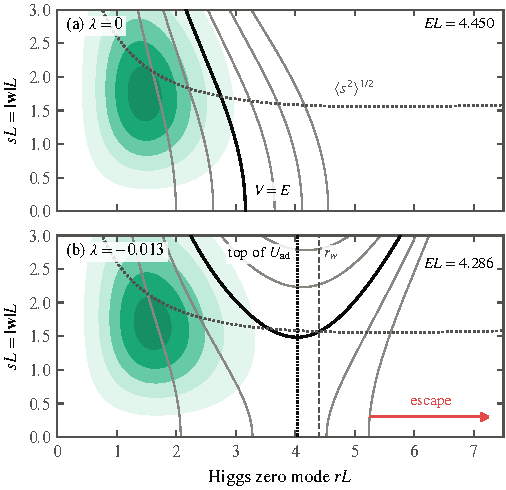
\includegraphics[width=0.7\textwidth]{prd_higgs_wavefunction}
\caption{Higgs and hypercharge zero modes in the two-dimensional model.
Filled contours: probability density of the lowest state in the $(r,s=|\bm w|)$ plane; thin lines: equipotentials of $V(r,s)$, the thick one at the eigenvalue $E$; dotted curve: transverse zero-point width $\langle s^2\rangle^{1/2}$.
(a)~$\lambda=0$: bound ground state.
(b)~$\lambda=-0.013$: quasi-bound state, computed with a wall at $r_w$ (dashed) beyond the top of the adiabatic barrier (dotted).
$V$ stays open at small $s$; the barrier comes from the zero-point energy of the gauge zero modes, and beyond its outer turning point the state escapes along $r$.} %
\label{fig:rb-wavefunction}
\end{figure}

\subsection{The finite-volume resonance as a multichannel Siegert state}
\label{sec:rb-siegert}

For $\lambda<0$ we solve $H_{\rm 2D}\psi=E\psi$ with complex $E=\varepsilon-i\Gamma/2$, where $\Gamma$ is the full width in conformal time (units $1/L$).
A Siegert state~\cite{Siegert:1939zz} is regular at the origin and purely outgoing at large $r$; it exists only at the discrete complex energies of the resonances, and $\Gamma$ is the decay rate of the quasi-stationary state.

\paragraph{Discretization and integration.}
In $s$ we use a sine discrete-variable representation on $(0,S_{\max})$, which builds in $v(0)=0$; in $r$ we integrate the matrix Numerov equation with renormalization.
We start at $r_0=0.01$ from the Frobenius solution $r^{s_0}(1+\alpha r/s_0)$, with $s_0=3/2$ for the two-dimensional model and $s_0=1.6726$ when $B_w\to3/(16r^2)$ is kept. %
At $R_{\rm out}=16$ we transform to the local adiabatic channels of $\bm w$, the eigenvectors of the $\bm w$ Hamiltonian at fixed $r$, and impose in each channel $m$ the outgoing (or, for closed channels, decaying) condition. %
For $u''+k^2(r)u=0$ the WKB solution $u\propto k^{-1/2}\exp(i\int^rk\,dr')[1+O(\hbar^2)]$ has the logarithmic derivative
\begin{equation}
\frac{u_m'}{u_m}=Y_m\equiv ik_m-\frac{k_m'}{2k_m}+\frac{i}{2k_m}\Bigl(\frac{3k_m'^2}{4k_m^2}-\frac{k_m''}{2k_m}\Bigr),
\label{eq:rb-siegert}
\end{equation}
to second order, with $k_m(r)=\{2[E-U_m(r)]\}^{1/2}$ and $U_m$ the adiabatic channel potential.
The resonance is a zero of the root function
\begin{equation}
f(E)=\det\bigl(u'_m-Y_mu_m\bigr),
\label{eq:rb-rootfn}
\end{equation}
evaluated on the matrix solution propagated from the origin.
We accumulate the determinant with a signed log-determinant, so that $f$ is an entire function of $E$, and we refine its zeros with Muller's method.

\paragraph{Locating the right zero.}
All channels are open in the outer region, so the phase of $f$ turns by about $N\,T_{\rm out}$ radians per unit energy, where $N$ is the number of channels and $T_{\rm out}$ the classical time in the outer region.
Muller iterations started with a wide step then converge onto Siegert zeros of box states of the $s$ direction, which move with $S_{\max}$, lie above the Born--Oppenheimer bracket, and have widths $0.7$--$1.3$. %
We therefore scan $|f|$ along the real axis in a window around the expected root, take the interior local minimum nearest the window centre, and start Muller there with a step of $0.001$. %
Every root is then recomputed with a larger $s$ box; a change $|\Delta E|>\max(2\times10^{-7},2\times10^{-3}\Gamma)$ flags a box state. %
This protocol is essential: an unguided search returns box zeros whose widths exceed the resonance width by orders of magnitude.

\begin{table}[t]
\centering
\caption{Static widths (units $1/L$) of the one-dimensional Born--Oppenheimer model, the two-dimensional model, and its Gaussian version 2D$_{\rm G}$, with the fixed couplings and the matching of Sec.~\ref{rep:h-matching}.} %
\label{tab:rb-widths}
\begin{tabular}{ccccc}
\toprule
$\lambda$ & $\Gamma_{\rm 1D}$ & $\Gamma_{\rm 2D}$ & $\Gamma_{\rm 2D}^{\rm G}$ & $\Gamma_{\rm 2D}/\Gamma_{\rm 1D}$ \\
\midrule
$-0.008$ & $2.010\times10^{-4}$ & $7.865\times10^{-5}$ & $1.032\times10^{-4}$ & $0.391$ \\ %
$-0.010$ & $9.871\times10^{-4}$ & $4.154\times10^{-4}$ & $5.318\times10^{-4}$ & $0.421$ \\ %
$-0.0143$ & $7.803\times10^{-3}$ & $3.774\times10^{-3}$ & $4.625\times10^{-3}$ & $0.484$ \\ %
\bottomrule
\end{tabular}
\end{table}

\paragraph{Convergence and independent methods.}
The widths converge fast (Table~\ref{tab:rb-widths}).
At $\lambda=-0.010$ and $-0.0143$, changing $(N,S_{\max})$ from $(32,14)$ to $(48,16)$ or $(24,12)$ changes $\Gamma$ by $2\times10^{-10}$, halving the step to $h=0.001$ by at most $8\times10^{-8}$, moving $R_{\rm out}$ to $14$ by $7\times10^{-7}$, and dropping the second-order terms of Eq.~(\ref{eq:rb-siegert}) by $3.4\times10^{-3}$, which measures the order of the outgoing condition. %
Three independent methods agree.
(i)~Finite differences with a complex absorbing potential (CAP) $-i\eta(r-7)^2\theta(r-7)$, with $\eta$ at the most stable point~\cite{Riss:1993cap}, give $\Gamma_{\rm 2D}/\Gamma_{\rm 1D,ex}=0.5313$ and $0.5317$ at grid steps $0.04$ and $0.03$, against $0.5303$ from the Siegert roots; the absolute CAP widths are low by $2.6\%$ in both models, which cancels in the ratio. %
In the final model the CAP pole agrees with the Siegert root to $0.08\%$ in $\Gamma$. %
(ii)~A real wall moved from $R_w=8$ to $11$ at $\lambda=-0.0143$ shows one level that stays at $\varepsilon=4.2737\pm0.002$ while the others cross it, matching the Siegert value $4.27375$. %
(iii)~For the one-dimensional model, exterior complex scaling~\cite{Simon:1979ecs} agrees with the Siegert root for the same inner boundary to $3\times10^{-9}$ in $E$ and $3\times10^{-7}$ relative in $\Gamma$. %
The CAP eigenvector has $P(r<5)=0.9988$ at $\lambda=-0.010$, and the probability beyond $0.75\,S_{\max}$ in $s$ is $10^{-10}$, so the resonance is localized in the well and the $s$ box plays no role. %

Two analytic limits check the solver.
A three-dimensional isotropic oscillator in the s wave gives $0.4500000000041$ against $0.45$ in a finite-element calculation, and the uncoupled limit $\Omega\equiv0.3$ separates to $8\times10^{-11}$. %
Over $\lambda=-0.004$ to $-0.020$ the Kemble WKB width agrees with the exact one to $3\%$ for tunneling exponents $S\approx2$--$25$. %
Changing the potential beyond $1.5$ times the outer turning point (linear tail, doubled quartic, frozen matching) changes $\Gamma$ by at most $0.75\%$, and beyond twice that radius by $10^{-4}$; the radial non-zero modes become tachyonic only at $r\approx31$. %

\paragraph{Mechanism.}
The resonance tunnels in $r$ through the barrier at $r\approx3$--$5.5$ while $\bm w$ stays in its local ground channel. %
At $\lambda=-0.010$ the resonance energy of the two-dimensional model lies $0.123/L$ below that of the one-dimensional model, $0.051$ from the gauge shape and $0.072$ from the $\bm w$ dynamics, while the barrier is unchanged. %
The width $\Gamma_{\rm 2D}=4.15\times10^{-4}$ lies between the Born--Oppenheimer values without and with $B_w$, $3.88\times10^{-4}$ and $7.99\times10^{-4}$, only $7\%$ above the first: nearly all of $B_w$ is spurious. %
The joint dynamics lowers the well and leaves the barrier unchanged, so that $\Gamma_{\rm 2D}/\Gamma_{\rm 1D}=0.39$--$0.48$ for $\lambda$ between $-0.008$ and $-0.0143$. %
The ratio decreases smoothly as $\lambda\to0^-$, because the barrier thickens and the same energy shift is amplified, and no $\lambda$-independent decay channel appears.

\paragraph{Inhomogeneous decay.}
Inhomogeneous decay is much slower than this homogeneous channel.
The scale-invariant instanton has action $8\pi^2/(3|\lambda|)\approx2.6\times10^3$ at $|\lambda|=0.01$~\cite{Andreassen:2017rzq}, compared with zero-mode tunneling exponents of $2$--$6$, and on the torus the non-zero modes turn tachyonic only far beyond the exit point. %

\subsection{Node-direct roots with running couplings}
\label{sec:rb-nodes}

For the hazard of Sec.~\ref{rep:h-survival} we solve the two-dimensional model directly at each node $\tau=0,0.5,\ldots,5$ of the turn and for each top mass on a grid of $0.2\GeV$. %
At each node we recompute the conditional Gaussian with the node couplings $g_2$ and $g_Y$, decompose it into $C_0$, $B_x$, and $\Omega_{\rm eff}^2$, evaluate $\Delta V_{\rm MC}$ with $(\lambda,g_2,g_Y,y_t)$ at $\mu(\tau)$, add the cross terms of Sec.~\ref{rep:h-cross}, and find the root.
No width ratio, interpolation in $\lambda$, or fitted correction enters.
The standard configuration is $N=24$, $S_{\max}=12$, $h=0.004$, $R_{\rm out}=16$. %
The root window is centred $0.0035$ below the root of the effective one-dimensional model at the same node, with half-width $0.012$ and scan step $0.0012$. %
In the runs with the earlier mapping all 377 two-dimensional columns passed the window and box tests at the first attempt, with $|\Delta E|\le1.4\times10^{-11}$ and relative changes of $\Gamma$ of at most $7.8\times10^{-5}$ under the box change, and the 220 columns of the run with the NNLO mapping passed in the same way. %
Relative to the configuration of Table~\ref{tab:rb-widths}, the standard configuration changes $\Gamma$ by at most $1.2\times10^{-6}$, $R_{\rm out}=14$ by $2.7\times10^{-6}$, and a zeroth-order outgoing condition by $3.0\times10^{-3}$; on the critical mass these are below $4\times10^{-7}$, $9\times10^{-7}$, and $1.0\times10^{-3}\GeV$. %
Eleven nodes instead of 29 change $m_c$ by $7\times10^{-5}\GeV$, and with the fixed couplings the node code reproduces the static widths of Table~\ref{tab:rb-widths} to $4.4\times10^{-6}$. %
These checks give the numerical item, $\pm0.002\GeV$, of the error budget (Sec.~\ref{rep:h-budget}); the full set of numerical controls is collected in Sec.~\ref{rep:v-convergence}. %

The two-dimensional model with the DMC shape was evaluated in three ways, by a ratio conversion of static widths, by an effective one-dimensional hazard, and by direct two-dimensional roots at every node; the last two change $m_c$ by only $0.011$ and $0.001\GeV$, so the numerical implementation of the reduced model has converged. %

\subsection{Full-dimensional validation and independent reimplementation: results}
\label{sec:rb-fulldim}

Section~\ref{rep:v-fulldim} describes the full-dimensional checks in detail; here we state the results that enter the error budget.
A Dirichlet wall at the gauge-invariant radius $|\bm\phi|=r_w$, between the barrier top and the outer classical turning point, is the only node of the walled ground state, so DMC for the full Hamiltonian in all sixteen coordinates has no fixed-node error.
The difference from the two-dimensional model with the same wall is $\Delta\varepsilon=-0.0032(8)$ at $\lambda=-0.010$ and $-0.0034(9)$ at $\lambda=-0.013$, independent of the wall position, and $-0.0043(9)$ at $\lambda=0$. %
The reduction error is thus a constant shift of the well by about $-0.0035/L$. %
With $d\ln\Gamma/d\varepsilon=7.6$ and $7.1$ from the two-dimensional model, $\Gamma_{\rm full}/\Gamma_{\rm 2D}=0.976$, and with the slopes $d\ln I/dm_t=5.269$, $3.218$, and $2.121\GeV^{-1}$ of the final hazard (Sec.~\ref{rep:h-survival}) %
\begin{equation}
\Delta m_c=-\frac{\ln(\Gamma_{\rm full}/\Gamma_{\rm 2D})}{d\ln I/dm_t}=+0.0046(11),\ +0.0075(19),\ +0.0115\GeV %
\label{eq:rb-dmc-conv}
\end{equation}
at $\Pone=0.9$, $1/2$, and $0.1$.
Three other estimates of the width ratio agree: multidimensional adiabatic WKB gives $0.937$ including $B_w$ under the barrier, the wall dependence of the tunneling tail gives $0.92(16)$ and $1.03(7)$, and a three-dimensional model with an SU(2) breathing mode gives $0.999$ (Fig.~\ref{fig:rb-gamma}). %
We carry the WKB envelope as a one-sided error, $+0.012$, $+0.020$, and $+0.031\GeV$ at $\Pone=0.9$, $0.5$, and $0.1$. %
Because $\Delta\varepsilon$ depends neither on the wall nor on $\lambda$, we apply the same ratio at every node and at $\Pone=0.1$, where $\lambda(\mub)=-0.0152$. %

The validation was done at fixed couplings and without the cross terms of Sec.~\ref{rep:h-cross}.
The cross terms stiffen the $\bm w$ direction and make it more adiabatic: the two-dimensional width exceeds that of the adiabatic one-dimensional reduction by only $1.0$--$1.8\%$ in the final model, against $6$--$8\%$ without cross terms, so the reduction is, if anything, more accurate in the final model. %
Within these assumptions the reduction moves the critical mass by at most $0.031\GeV$. %
An independent blind reimplementation of the chain without cross terms, with the earlier Standard Model mapping, reproduces its critical masses to $0.005\GeV$ (Sec.~\ref{rep:v-blind}). %

\begin{figure}[t]
\centering
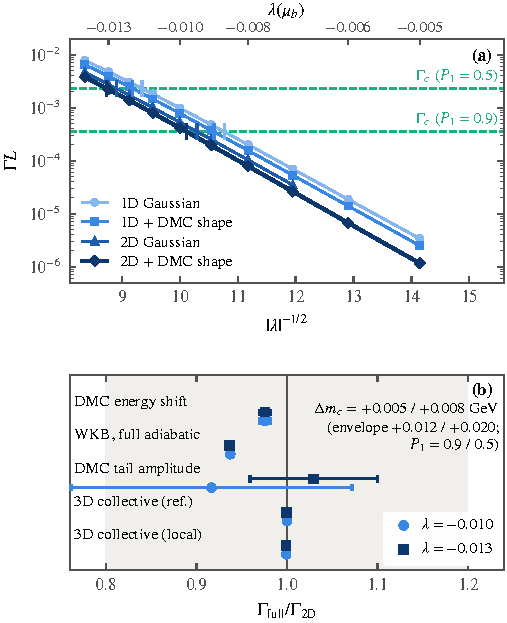
\includegraphics[width=0.66\textwidth]{prd_gamma_validation}
\caption{Resonance widths of the reduced models and their full-dimensional check.
(a)~$\Gamma L$ against $|\lambda|^{-1/2}$ for one- and two-dimensional models with Gaussian or DMC gauge shape; the straight lines on the logarithmic scale are the WKB form $\ln\Gamma=a-b|\lambda|^{-1/2}$.
Dashed: the constant widths $\Gamma_c=-\ln\Pone/\eta_\infty$ that give $\Pone=0.5$ and $0.9$; ticks: where each model reaches them.
(b)~$\Gamma_{\rm full}/\Gamma_{\rm 2D}$ at $\lambda=-0.010$ and $-0.013$ from four estimators; all lie within $20\%$ (band) and would raise $m_c$ by $+0.005$ and $+0.008\GeV$ at $\Pone=0.9$ and $0.5$, a shift not included in the central values (one-sided envelope $+0.012$ and $+0.020\GeV$).} %
\label{fig:rb-gamma}
\end{figure}

\subsection{The size of the threshold}
\label{sec:rb-size}

The threshold $\lamc\approx-0.01$ follows from three ingredients: the WKB form of the width, the duration of the turn, and the residual linear confinement after the matching.
Figure~\ref{fig:rb-threshold}(a) shows the effective potential along $r$ near threshold.

\paragraph{WKB exponent of a linearly confined quartic runaway.}
For $U(r)=\sigma r-|\lambda|r^4/4$ and an energy well below the barrier, the outer turning point is $r_0=(4\sigma/|\lambda|)^{1/3}$, and with $r=r_0x$ one has $U=\sigma r_0\,x(1-x^3)$.
The tunneling exponent is
\begin{equation}
S=2\int_0^{r_0}\!\sqrt{2U}\,dr=2\sqrt{2\sigma}\,r_0^{3/2}\int_0^1x^{1/2}(1-x^3)^{1/2}dx=\frac{2\pi\sqrt2}{3}\frac{\sigma}{|\lambda|^{1/2}}\simeq2.962\,\frac{\sigma}{|\lambda|^{1/2}}, %
\label{eq:rb-wkb}
\end{equation}
where the substitution $x^3=v$ turns the integral into $\frac13B(\frac12,\frac32)=\pi/6$ and $r_0^{3/2}=2\sigma^{1/2}|\lambda|^{-1/2}$.
The width therefore obeys $\ln\Gamma=a-b|\lambda|^{-1/2}$ with $b=2.962\,\sigma$. %
Fits to the nodal widths give $b=1.31$--$1.38$ (at $\tau=0$: $a=5.91$, $b=1.307$; the static box at $\mub$ gives $a=\aFitA$ and $b=\bFitA$ for $\lamFitLo\le\lambda\le\lamFitHi$, Sec.~\ref{sec:v11-static-box}), with root-mean-square residuals $0.05$--$0.09$ in $\ln\Gamma$; a three-parameter form $a-b|\lambda|^{-p}$ gives $p=0.74$ at $\tau=0$ and $0.55$ at $\tau=5$, because the local exponent flattens as the resonance approaches the barrier top. %

\paragraph{Hazard form.}
The hazard of Sec.~\ref{rep:h-survival} integrates $\Gamma$ over the conformal duration $\eta_\infty$ of one branch.
We define the effective exponent of the hazard by its logarithmic derivative at threshold,
\begin{equation}
b_{\rm eff}\equiv2|\lamc|^{3/2}\Bigl|\frac{d\ln I}{d\lambda(\mub)}\Bigr|=1.40,\ 1.30,\ 1.19 %
\label{eq:rb-beff}
\end{equation}
at $\Pone=0.9$, $0.5$, and $0.1$, from $d\ln I/d\lambda(\mub)=-805$, $-488$, and $-319$. %
Up to a slowly varying prefactor, $I\simeq A_{\rm eff}\,\eta_\infty\exp(-b_{\rm eff}|\lambda|^{-1/2})$, with $\lambda\equiv\lambda(\mub)$.
The effective slope $\sigma_{\rm eff}=b_{\rm eff}/2.962=0.44$ at $\Pone=1/2$ ($0.47$ and $0.40$ at $\Pone=0.9$ and $0.1$) is about one third of the zero-point slope $\sigma_0=1.31$ of Eq.~(\ref{eq:rb-linear}): in the reduced model the zero-point energy rises with slope $\zpSlopeLo$--$\zpSlopeHi$ rather than $\sigma_0$ at $r=1$--5 (Sec.~\ref{sec:v11-static-box}), the WKB form absorbs the finite height of the barrier, and the one-loop energy of the non-zero modes lowers the local slope by $10$--$33\%$ at $r=1$--5 and roughly halves the barrier above the resonance level, without removing the confinement. %
In the reduced model of Fig.~\ref{fig:rb-threshold}(a), without cross terms, and for the radial potential including the centrifugal term $3/(8r^2)$, the barrier above the resonance level falls from $1.565/L$ to $0.715/L$ for $\lambda=-0.010$ and from $1.211/L$ to $0.534/L$ for $\lambda=-0.013$ when the matching is included. %
The matching combines the destabilizing tadpole of the periodic bosons (Sec.~\ref{sec:rb-tower}) with the stabilizing one of the antiperiodic top tower (Sec.~\ref{sec:rb-rg}), and the hypercharge zero mode, pinned by the antiperiodic fermions (Sec.~\ref{rep:h-cross}), also enters $\sigma_{\rm eff}$. %

\paragraph{Closed form for the threshold.}
Setting $I=\ln2$ (that is, $\Pone=1/2$) gives
\begin{equation}
|\lamc|^{1/2}\simeq\frac{b_{\rm eff}}{\ln(A_{\rm eff}\,\eta_\infty/\ln2)} .
\label{eq:rb-lamc-size}
\end{equation}
The effective prefactor $A_{\rm eff}\simeq310$ absorbs the energy of the resonance ($\varepsilon\approx4.3/L$), the shape of the barrier, and the reduction of the width by the running along the turn; it is fixed by reproducing the computed threshold and is not universal. %
With $b_{\rm eff}=1.30$ and $\eta_\infty=299.8$, this value of $A_{\rm eff}$ returns $\lamc=-0.0121$ by construction; the content of the formula is the logarithmic dependence, checked directly in Sec.~\ref{rep:h-universality}. %
The running matters at the level of the effective duration: holding the $\tau=0$ width for the whole branch would overestimate the hazard, and $I/(\Gamma(0)\eta_\infty)=0.77$, $0.82$, and $0.87$ at the three levels. %
The duration and the prefactor enter only through the logarithm: doubling or halving $\eta_\infty$ changes $|\lamc|$ by $-11\%$ or $+13\%$, and changing $g_2$, $g_Y$, or $y_t$ by $10\%$ changes it by $6.6\%$, $1.6\%$, or $6.3\%$, so the magnitude $\lamc\approx-0.01$ is fixed to within a factor of about $1.2$. %
The effective exponent at threshold, $S_c=b_{\rm eff}/|\lamc|^{1/2}=14.7$, $11.8$, and $9.7$ at the three levels, is moderate, which is why the threshold is sharp in $\lambda$ but not in $\Pone$. %
It is the exponent of this effective law, whose prefactor $A_{\rm eff}\simeq310$ absorbs a factor of order $e^6$; the WKB barrier action is smaller, $4.3$ at the static threshold $\lamc(300)$ (Sec.~\ref{sec:v11-mechanism-context}). %
The dependence on the duration and on the couplings is worked out in Sec.~\ref{rep:h-universality}.

\begin{figure}[t]
\centering
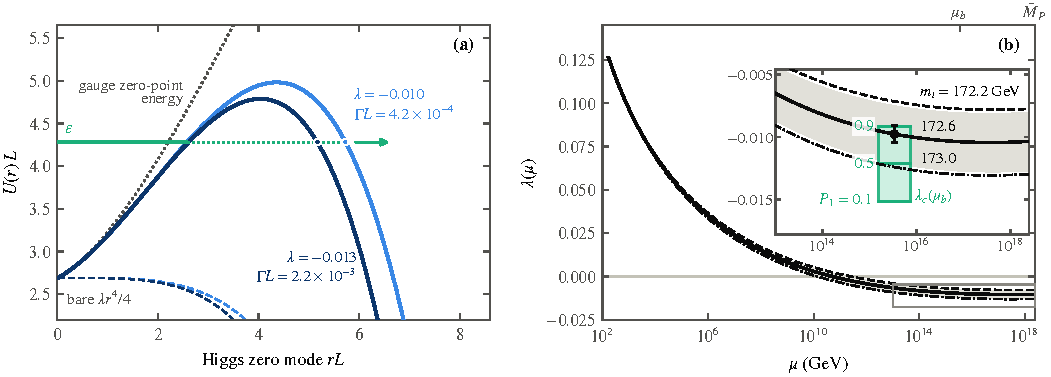
\includegraphics[width=\textwidth]{prd_threshold}
\caption{Finite-volume threshold of the Higgs zero mode.
(a)~Effective potential along $r$ for $\lambda=-0.010$ and $-0.013$ (reduced model without cross terms or centrifugal term): the zero-point energy of the gauge zero modes (dotted), lowered by the non-zero modes, holds back the negative quartic (dashed), so the state is a resonance at $\varepsilon$ with width $\Gamma$ (dots: outer turning points). %
(b)~Running quartic coupling $\lambda(\mu)$ for $m_t=172.2$ (dashed), $172.6$ (solid), and $173.0\GeV$ (dash-dotted), with the band from $\alpha_s(M_Z)=0.1180\pm0.0009$; inset: the hazard-equivalent threshold $\lamc(\mub)$ for $\Pone=0.9$, $0.5$, and $0.1$, and the Standard Model value with its mapping uncertainty (Sec.~\ref{rep:h-smmap}).} %
\label{fig:rb-threshold}
\end{figure}

\subsection{The confinement mechanism in field-theory context}
\label{sec:v11-mechanism-context}

The confinement of the Higgs zero mode rests on one term, the zero-point energy of the constant $W$ and $Z$ modes at fixed $r$, which grows linearly with $r$.
This subsection relates that term to known structures of small-volume gauge theory, matrix models and thermal field theory, states which fields can cancel it, and compares the resonance with the decay channels of a small compact space, with inhomogeneous tunnelling and with Planck-suppressed operators.
Numbers refer to the static box of Sec.~\ref{sec:v11-static-box}; its box~A has the Standard Model couplings at $\mu=\mub$ for $m_t=172.60\GeV$, which are those of the first node of the turn. %
The fit window is the range $\lamFitLo\le\lambda\le\lamFitHi$ in which Sec.~\ref{sec:v11-static-box} fits the widths of box~A with Eq.~(\ref{eq:rb-wkb}), and $\kappa$ is the factor by which Sec.~\ref{sec:v11-kappa} multiplies the couplings of the gauge zero modes. %

\paragraph{A linear term from the constant gauge modes.}
At fixed $r$ the mass matrix of Eq.~(\ref{eq:rb-massmatrix}) makes the constant $W$ and $Z$ modes oscillators of frequencies $g_2r/2$ and $g_Zr/2$, whose zero-point energy rises as $\sigma_0r$ with $\sigma_0=\frac32g_2+\frac34g_Z$ [Eq.~(\ref{eq:rb-linear})]; with the couplings of box~A, $\sigma_0=1.31$. %
Since $r=(2\Phi^\dagger\Phi)^{1/2}$, the term is linear in $|\Phi|$ and not analytic in $\Phi^\dagger\Phi$.
It plays the role of the zero-point energy along the classically flat valleys of a quartic potential.
At $\lambda=0$ the potential of Eq.~(\ref{eq:rb-H0}) vanishes along the whole Higgs direction $\bm x=\bm w=0$, and the zero-point energy of the transverse gauge modes closes this valley, as it makes the spectrum of $p_x^2+p_y^2+x^2y^2$ discrete although the classically allowed region extends to infinity along the axes~\cite{Simon:1983jy}.
In SU(2) Yang--Mills theory on a small torus the same mechanism gives an abelian constant mode $C$ the conical potential $2|C|/L$ (in the normalization of Ref.~\cite{vanBaal:2000zc}), the zero-point energy of the four charged constant modes of frequency $|C|/L$ transverse to it~\cite{vanBaal:2000zc,Barbon:2005zj}, and it makes the spectra of the bosonic membrane and of bosonic matrix models discrete~\cite{deWit:1988xki,Barbon:2005zj}. %
The Higgs zero mode differs from these examples in that its valley falls as $-|\lambda|r^4/4$ for $\lambda<0$, so the linear term holds the zero mode only up to the barrier at $r_{\rm top}=(\sigma/|\lambda|)^{1/3}$ (Sec.~\ref{sec:rb-H0}), and the bound state of the valley becomes the resonance of Sec.~\ref{sec:rb-siegert}.

\paragraph{Relation to the thermal cubic term.}
The linear term is the finite-volume counterpart, with the opposite sign, of the term cubic in the gauge-boson masses that the static Matsubara modes add to the effective potential at finite temperature~\cite{Dine:1992wr,Arnold:1992rz}.
Both terms come from bosonic modes that have no gap from the compact directions.
Such a mode of a real boson of mass $m$ is integrated only over its $d$ non-compact Euclidean directions, and in dimensional regularization
\begin{equation}
\frac12\int\!\frac{d^dk}{(2\pi)^d}\,\ln\bigl(k^2+m^2\bigr)=-\frac{\Gamma(-d/2)}{2\,(4\pi)^{d/2}}\,m^d
=\begin{cases}+\dfrac{m}{2}, & d=1,\\[8pt] -\dfrac{m^3}{12\pi}, & d=3,\end{cases}
\label{eq:v11-gapless}
\end{equation}
which follows from $\int d^dk\,(2\pi)^{-d}(k^2+m^2)^{-1}=\Gamma(1-d/2)\,m^{d-2}/(4\pi)^{d/2}$ by integration in $m^2$, with $\Gamma(-\frac12)=-2\sqrt\pi$ and $\Gamma(-\frac32)=\frac43\sqrt\pi$.
At temperature $T$ the free-energy density of the field is $T\sum_n\frac12\int d^3k\,(2\pi)^{-3}\ln(\omega_n^2+k^2+m^2)$ with $\omega_n=2\pi nT$.
The static mode $n=0$ is a three-dimensional field and contributes $-Tm^3/(12\pi)$, while the modes with $n\neq0$ have the gap $2\pi T$ and are analytic in $m^2$ for $|m|<2\pi T$~\cite{Dine:1992wr}.
In the box at zero temperature the energy is $\frac12\sum_{\bm k}\omega_{\bm k}=\sum_{\bm k}\frac12\int dk_0\,(2\pi)^{-1}\ln(k_0^2+\bm k^2+m^2)$.
The constant mode $\bm k=0$ is a quantum oscillator and contributes $+m/2$, while the modes with $\bm k\neq0$ have the gap $2\pi/L$ and give the energy $E_{\rm std}$ of Eq.~(\ref{eq:rb-Estd}), analytic in $m^2$ for $|m|<2\pi/L$.
For the electroweak gauge bosons the counting is the same in both cases, six $W$ and three $Z$ modes, from the three polarizations of each massive vector at finite temperature and from the three spatial directions of each constant mode in the box, so that
\begin{equation}
\Delta V_T\supset-\frac{T}{12\pi}\bigl(6m_W^3+3m_Z^3\bigr),\qquad
L\,\Delta E_{\rm box}=\frac L2\bigl(6m_W+3m_Z\bigr)=\sigma_0r,
\label{eq:v11-cubic-linear}
\end{equation}
with $m_W=g_2r/(2L)$ and $m_Z=g_Zr/(2L)$ in the box.
The first expression is the leading cubic term of the thermal potential, before the resummation of the static modes~\cite{Arnold:1992rz}, and the second is Eq.~(\ref{eq:rb-linear}).
The sign is that of $-\Gamma(-d/2)$, positive for $d=1$ and negative for $d=3$: the constant spatial modes are quantum oscillators with positive zero-point energy, whereas the one-loop energy of the three-dimensional static field is negative.
The roles differ accordingly: at finite temperature the negative cubic term produces the barrier of a first-order transition between the symmetric and the broken phase; in the box the positive linear term holds the zero mode at the origin against the negative quartic.

Terms proportional to $(m^2)^{d/2}$ with odd $d$ are non-analytic in $\Phi^\dagger\Phi$~\cite{Barbon:2006us}.
The infinite-volume effective potential at zero temperature contains no odd power of $m$: every mode is integrated over four non-compact directions, and the same integral gives, after $\MSbar$ subtraction, the Coleman--Weinberg term of Eq.~(\ref{eq:rb-VCW}), whose logarithm is the only non-analyticity of that potential.
For masses large compared with the gap the gapped modes cancel the non-analytic term again: in the box $D_P(m^2)\to-m/2+0.8375$ for $mL\gg2\pi$ (Sec.~\ref{sec:rb-tower}). %
Antiperiodic fermions have no mode without a gap, since their lowest momentum is $\sqrt3\,\pi/L$ in the box and $\pi T$ at finite temperature, so they give no such term; in the box they enter only through the matching potential, which is analytic in $\tilde m_t^2$ for $|\tilde m_t|<\sqrt3\,\pi/L$ (Sec.~\ref{sec:rb-tower}).

\paragraph{Constant fermion modes.}
Constant fermion modes act against the confinement.
If all three cycles of the torus are periodic, as for the torus of Ref.~\cite{Fornal:2026qfq}, every fermion has a constant mode at trivial holonomy; an SU(3) center holonomy twists the quarks by $\pm\frac13$ and removes their constant modes, and that sector is not analysed (Sec.~\ref{sec:rb-spin}). %
For the top quark at fixed $r$ its Hamiltonian is $\tilde m_t\,\psi_0^\dagger\gamma^0\psi_0$, summed over the three colours, with $\tilde m_t=y_tr/\sqrt2$ [Eq.~(\ref{eq:rb-masses})], and $\gamma^0$ has the eigenvalues $\pm1$, each twice degenerate.
In the charge-conjugation symmetric ordering each of the $4\times3$ levels of energy $\pm\tilde m_t$ contributes $-\tilde m_t/2$ to the ground-state energy, the filled negative levels through $\varepsilon/2$ and the empty positive ones through $-\varepsilon/2$, so that
\begin{equation}
E_t^{(0)}=-12\cdot\frac{\tilde m_t}{2}=-6\tilde m_t=-\frac{6y_t}{\sqrt2}\,r\simeq-1.82\,r,
\label{eq:v11-top-zero}
\end{equation}
with $y_t(\mub)=0.428$ of box~A. %
The factor $12$ is the weight with which the top quark enters the one-loop matching (Sec.~\ref{sec:rb-rg}).
The term exceeds $\sigma_0r=1.31\,r$, so the net linear term of the constant modes would be negative, $(1.31-1.82)\,r$, and the zero-point confinement would fail; the lighter fermions add terms smaller by their Yukawa couplings. %
This statement is qualitative: at large $r$ the non-zero modes of both towers cancel the constant-mode terms (Sec.~\ref{sec:rb-tower}), and at trivial holonomy the fully periodic torus does not turn around (Sec.~\ref{sec:rb-spin}).
It parallels the supermembrane, in which the fermionic zero-point energy cancels the bosonic one along the valleys and the spectrum becomes continuous~\cite{deWit:1988xki}.
With one antiperiodic cycle or more the fermions have no constant modes (Sec.~\ref{sec:rb-spin}), and nothing cancels the confinement by the gauge zero modes.

\paragraph{Uniform tunnelling in a small compact space.}
A small compact volume speeds up vacuum decay: when the volume is small, a uniform tunnelling mode replaces the bubble~\cite{Hassan:2026cmp}, and the Schwinger effect in small compact directions proceeds through a homogeneous channel~\cite{Brown:2015kgj}; thin-wall decay with one compact dimension has been analysed for a scalar field~\cite{Antoniadis:2024ent}.
These analyses treat a scalar field with a barrier of its own or the Schwinger discharge of an electric field; in none of them do gauge zero modes confine a scalar zero mode.
For the Higgs field at $\lambda<0$ the uniform mode has no barrier of its own.
With the couplings of the gauge zero modes switched off ($\kappa=0$ in Sec.~\ref{sec:v11-kappa}) its radial potential, $3/(8r^2)+\lambda r^4/4+\Delta V_{\rm MC}(r)$, falls monotonically for every $\lambda$ between $-0.04$ and $0$, and the zero mode has no narrow (quasi-bound) resonance. %
When space is a three-torus the gauge zero modes supply the barrier.
The decay of the electroweak state in the box is still much faster than bubble nucleation in infinite volume, as the next paragraph shows, but it is tunnelling with a finite width rather than a classical roll.

\paragraph{Inhomogeneous tunnelling.}
Section~\ref{sec:rb-siegert} compared the action of the scale-invariant bounce with the zero-mode tunnelling exponents $2$--$6$ of the earlier model.
In the static box at $\mub$ the WKB exponents across the barrier are $2.1$--$7.9$ in the fit window $\lamFitLo\le\lambda\le\lamFitHi$ of Sec.~\ref{sec:v11-static-box}, and $3.1$, $4.3$, $7.8$ and $12.5$ at the thresholds $\lamc(N)$ for $N=10^2$, $3\times10^2$, $10^4$ and $10^6$. %
The Fubini-type bounce of a negative quartic has the action $8\pi^2/(3|\lambda|)$ for every radius~\cite{Andreassen:2017rzq}, which is $1.8\times10^3$, $2.2\times10^3$, $3.7\times10^3$ and $5.9\times10^3$ at these thresholds, at least $450$ times the zero-mode exponent. %
For the Standard Model couplings, a bounce of radius $R<L$ probes $\lambda$ at scales above $1/L$, where $\lambda(\mu)\ge-0.0104$ for $m_t=172.6\GeV$, with the minimum near $4\times10^{17}\GeV$; its action is therefore at least $2.5\times10^3$, and at least $2.0\times10^3$ for $m_t=173.0\GeV$. %
Inhomogeneous decay is therefore negligible against the zero-mode channel for every duration considered here.

\paragraph{Planck-suppressed operators.}
The width depends on the potential only up to the outer turning point of the barrier, $r_{\rm out}=5.3$--$5.7$ in box~A for $\lamc(300)\le\lambda\le\lambda_{\rm SM}(\mub)$ and $6.4$ at $\lamc(10^4)$, that is, on field values $r\lesssim6$, or $\phi=r/L\lesssim0.008\,\MPbar$ at $\mub=\MPbar/722$. %
A term $c\,\phi^6/\MPbar^2$ in the potential adds $c\,r^6(\mu/\MPbar)^2$ to $LH$ at $\mu=1/L$, which acts as a shift of the quartic coupling by $\Delta\lambda_{\rm eff}(r)=4c\,r^2(\mu/\MPbar)^2$.
At $\mub$ and $r=6$ this is $2.8\times10^{-4}c$ ($2.2\times10^{-4}c$ and $2.5\times10^{-4}c$ at $r=5.3$ and $5.7$). %
Through $d\lambda(\mub)/dm_t\approx-0.0066\GeV^{-1}$ (Sec.~\ref{rep:h-smmap}) it raises the critical top mass by at most about $0.04c\GeV$ for $c>0$, which is below the Standard Model error of the criterion, $\pm0.10\GeV$, for $|c|\lesssim2$. %
Higgs-coupled states of mass $M$ between $2\pi\mub$ and $\MPbar$ would generate the same operator with $\MPbar$ replaced by $M$, which shifts the critical mass by about $0.042c\,(\MPbar/M)^2\GeV$; the magnitude of this shift stays below $0.10\GeV$ only for $M\gtrsim0.65\,|c|^{1/2}\MPbar$, so the criterion also assumes that such states, if present, lie near $\MPbar$ or couple weakly to the Higgs field. %
